\documentclass[border=6pt]{standalone}
\usepackage{amsmath,amssymb}
\usepackage{tikz}
\usetikzlibrary{shapes.geometric, arrows.meta, positioning, fit, calc}
\begin{document}
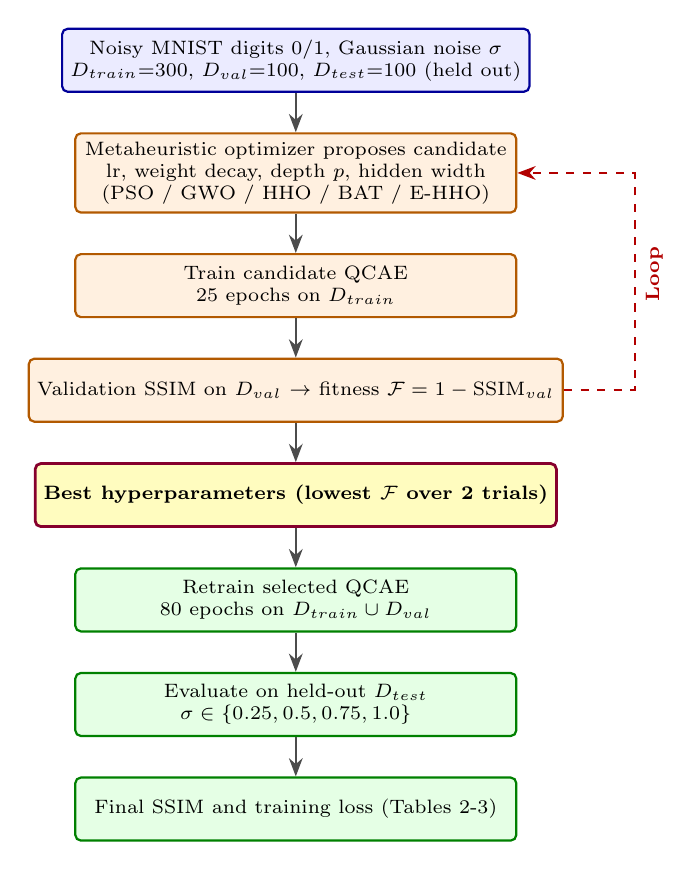
\begin{tikzpicture}[
    node distance=5mm and 5mm,
    data/.style={rectangle, rounded corners=2pt, draw=blue!60!black, line width=0.8pt, align=center, minimum width=5.6cm, minimum height=0.8cm, font=\scriptsize, fill=blue!8, inner sep=3pt},
    loopblk/.style={rectangle, rounded corners=2pt, draw=orange!70!black, line width=0.8pt, align=center, minimum width=5.6cm, minimum height=0.8cm, font=\scriptsize, fill=orange!12, inner sep=3pt},
    bestblk/.style={rectangle, rounded corners=2pt, draw=purple!70!black, line width=1pt, align=center, minimum width=5.6cm, minimum height=0.8cm, font=\scriptsize\bfseries, fill=yellow!25, inner sep=3pt},
    finalblk/.style={rectangle, rounded corners=2pt, draw=green!50!black, line width=0.8pt, align=center, minimum width=5.6cm, minimum height=0.8cm, font=\scriptsize, fill=green!10, inner sep=3pt},
    arr/.style={-Stealth, thick, black!70},
    looparr/.style={-Stealth, thick, red!70!black}
]
\node[data] (data) {Noisy MNIST digits 0/1, Gaussian noise $\sigma$\\$D_{train}$=300, $D_{val}$=100, $D_{test}$=100 (held out)};
\node[loopblk, below=of data] (search) {Metaheuristic optimizer proposes candidate\\lr, weight decay, depth $p$, hidden width\\(PSO / GWO / HHO / BAT / E-HHO)};
\node[loopblk, below=of search] (traincand) {Train candidate QCAE\\25 epochs on $D_{train}$};
\node[loopblk, below=of traincand] (valfit) {Validation SSIM on $D_{val}$ $\rightarrow$ fitness $\mathcal{F}=1-\mathrm{SSIM}_{val}$};
\node[bestblk, below=of valfit] (best) {Best hyperparameters (lowest $\mathcal{F}$ over 2 trials)};
\node[finalblk, below=of best] (retrain) {Retrain selected QCAE\\80 epochs on $D_{train}\cup D_{val}$};
\node[finalblk, below=of retrain] (test) {Evaluate on held-out $D_{test}$\\$\sigma \in \{0.25, 0.5, 0.75, 1.0\}$};
\node[finalblk, below=of test] (report) {Final SSIM and training loss (Tables 2-3)};

\draw[arr] (data) -- (search);
\draw[arr] (search) -- (traincand);
\draw[arr] (traincand) -- (valfit);
\draw[arr] (valfit) -- (best);
\draw[arr] (best) -- (retrain);
\draw[arr] (retrain) -- (test);
\draw[arr] (test) -- (report);

\coordinate (loopbend) at ($(valfit.east)+(0.9,0)$);
\draw[looparr, dashed] (valfit.east) -- (loopbend) |- (search.east);
\node[font=\scriptsize\bfseries, align=left, text=red!70!black, anchor=west, rotate=90] at ($(loopbend)+(0.25,1.0)$) {Loop};
\end{tikzpicture}
\end{document}
